\documentclass[tikz,border=15pt]{standalone}
\usepackage{circuitikz}
\begin{document}
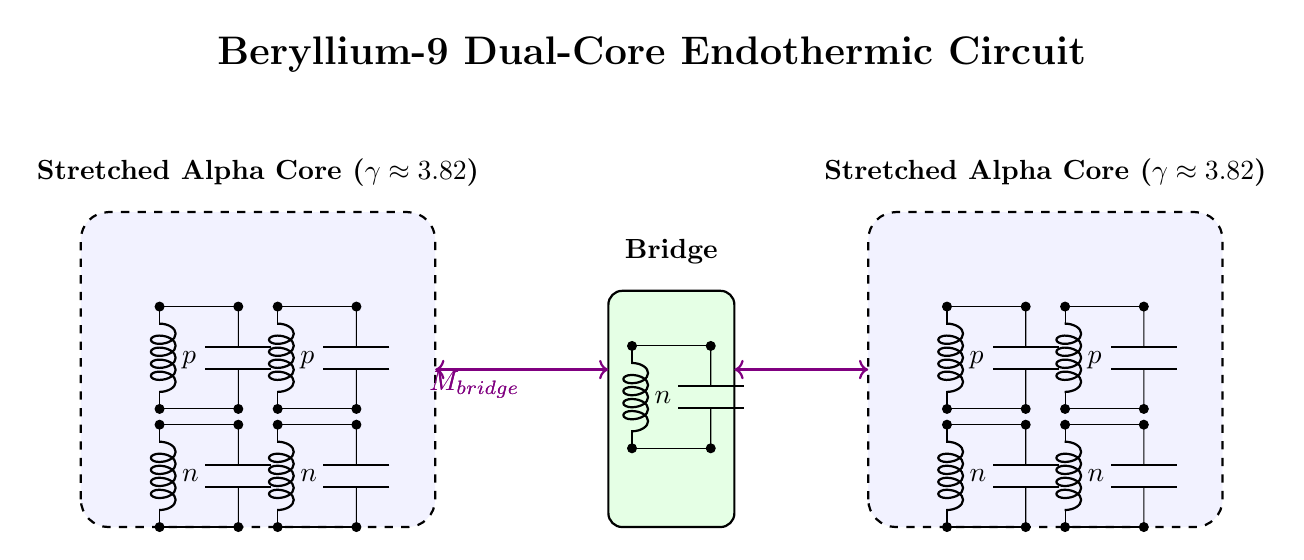
\begin{tikzpicture}
    \def\tank#1#2#3{
        \begin{scope}[shift={(#1)}]
            \draw (0,0.3) to[L=$#3$, *-*] (0,-1.0);
            \draw (1,0.3) to[C, *-*] (1,-1.0);
            \draw (0,0.3) -- (1,0.3);
            \draw (0,-1.0) -- (1,-1.0);
        \end{scope}
    }
    
    % Alpha Core 1 (Left)
    \draw[rounded corners=10pt, fill=blue!5, thick, dashed] (-5,-1.5) rectangle (-0.5,2.5);
    \node at (-2.75, 3) {\textbf{Stretched Alpha Core ($\gamma \approx 3.82$)}};
    
    \tank{-4,1}{1}{p}
    \tank{-2.5,1}{2}{p}
    \tank{-4,-0.5}{3}{n}
    \tank{-2.5,-0.5}{4}{n}
    
    % Alpha Core 2 (Right)
    \draw[rounded corners=10pt, fill=blue!5, thick, dashed] (5,-1.5) rectangle (9.5,2.5);
    \node at (7.25, 3) {\textbf{Stretched Alpha Core ($\gamma \approx 3.82$)}};
    
    \tank{6,1}{5}{p}
    \tank{7.5,1}{6}{p}
    \tank{6,-0.5}{7}{n}
    \tank{7.5,-0.5}{8}{n}
    
    % Bridge Neutron (Center)
    \draw[rounded corners=5pt, fill=green!10, thick] (1.7,-1.5) rectangle (3.3,1.5);
    \node at (2.5, 2) {\textbf{Bridge}};
    \tank{2.0,0.5}{9}{n}
    
    % Endothermic Coupling (Tension)
    \draw[<->, violet, thick, out=0, in=180] (-0.5, 0.5) to (1.7, 0.5) node[midway, above] {$M_{bridge}$};
    \draw[<->, violet, thick, out=180, in=0] (5, 0.5) to (3.3, 0.5) node[midway, above] {$M_{bridge}$};
    
    \node at (2.25, 4.5) {\Large \textbf{Beryllium-9 Dual-Core Endothermic Circuit}};
\end{tikzpicture}
\end{document}
